\chapter{Statistiques quantiques}



\section{Pauli et les statistiques}


On a pu observer avec le paradoxe de Gibbs qu'il est dangereux d'oublier le caractère quantique des particules. Pour le moment on a pu traiter le problème du caractère indiscernable avec le $\frac{\xi^N}{N!}$. Les complications induites par la difficulté de calculer des sommes discrètes nous ont poussé à essayer d'utiliser l'approximation classique pour transformer les sommes en intégrales. On a ainsi négligé la quantification des niveaux d'énergie.

\subsection{Bosons et fermions}

On rappelle que l'on a vu 2 grandes familles de particules qui ont chacune un comportement particulier suite à une permutation quelconque de 2 particules

\begin{itemize}[label=\ding{69}]

	\item Les bosons, la symétrie : 

	$$\varphi_{bosons}(\vec{r_1},...\vec{r_i},\vec{r_j},...,\vec{r_N})=\varphi_{bosons}(\vec{r_1},...\vec{r_j},\vec{r_i},...,\vec{r_N})$$

	\item Les fermions, l'anti-symétrie :

	$$\varphi_{bosons}(\vec{r_1},...\vec{r_i},\vec{r_j},...,\vec{r_N})=-\varphi_{bosons}(\vec{r_1},...\vec{r_j},\vec{r_i},...,\vec{r_N})$$

\end{itemize}

Pour passer à l'analyse de la physique statistique on va présenter tout de même l'ensemble dans lequel on va travailler. On travaille dans une représentation Grand canonique pour prendre en compte le nombre de particules par niveau. Cependant nous utiliserons une astuce, nous prendrons un nombre de particules suffisamment élevé pour que $\bar{N}=N$. On a donc plus vraiment de variation de particules et $\mu$ devient un facteur de normalisation que l'on calculera à partir du nombre de particules.


\section{Bosons: "statistique de Panurge"}


On se rend compte qu'il est impossible de sommer sur tous les états comme on antérieurement si l'on prend en compte le caractère anti-symétrique. On procède donc différemment, sommons  sur le nombre de particules pour chacune d'entre elles. C'est à dire:
$$\Xi_b= \sum_{\{N_i\}}e^{-\beta \sum_i N_i (\epsilon_i-\mu)}$$
Un exemple pour faciliter la compréhension. \\
Soit un ensemble de particules avec 2 niveaux d'énergie $E_1,E_2$ qui peuvent être peuplés par 2 et 1 particules respectivement.
$$\Xi_b= \sum_{\{N_1\},\{N_2\}}e^{-\beta \sum_i^2 N_i (\epsilon_i-\mu)}=\sum_{N_1=\{0,1,2\}}e^{-\beta N_1 (\epsilon_1-\mu)}\sum_{N_2=\{0,1\}}e^{-\beta  N_2 (\epsilon_2-\mu)}=$$
$$\left(1+e^{-\beta  (\epsilon_1-\mu)}+e^{-\beta  2(\epsilon_1-\mu)}\right)\left(1+e^{-\beta  (\epsilon_1-\mu)}\right)$$
Prenons désormais le cas d'intérêt, les bosons, il est important de comprendre que pour les bosons il n'y a pas de limite par état puis qu'ils peuvent co-exister dans un même état. En réécrivant $\Xi_b$
$$\Xi_b= \sum_{\{N_i\}}e^{-\beta \sum_i N_i (\epsilon_i-\mu)}=\prod_i\sum_{N_i}e^{-\beta N_i (\epsilon_i-\mu)}$$
On se rend compte que si N grand, ce que l'on à déjà stipulé antérieurement on peut considérer $N\rightarrow\infty$ et donc utiliser la formule de la somme d'une série géométrique.
$$\Xi_b=\prod_i\frac{1}{1-e^{-\beta N_i (\epsilon_i-\mu)}}$$
Il faut évidemment que $\mu < \epsilon_0\leq \epsilon_i$
On calcule donc le nombre moyen de particules :
$$\bar{N}=\frac{1}{\beta}\frac{\partial ln(\Xi_b)}{\partial \mu}=\sum_i \frac{1}{e^{-\beta (\epsilon_i-\mu)}-1}=\sum_i\bar{N_i}$$


\section{Les fermions: "une politique d'exclusion"}


On va procéder de manière identique cependant on va prendre en compte le fait qu'au maximum $2s+1$ particules peuvent se trouver dans un état énergétique, avec s le spin.Cependant dans un premier temps on ne le prendra pas en compte, on suppose donc qu'il peut y avoir 0 ou 1 particule par niveau énergétique.
On l'applique à :
$$\Xi_f=\prod_i\sum_{N_s}e^{-\beta N_s (\epsilon_i-\mu)}=\prod_i\left(1+e^{-\beta  (\epsilon_i-\mu)}\right)$$
Et donc:
$$\bar{N}=N=\frac{1}{\beta}\frac{\partial ln(\Xi_b)}{\partial \mu}=\sum_i \frac{1}{e^{-\beta (\epsilon_i-\mu)}+1}=\sum_i\bar{N_i}$$


\section{La limite classique}


\subsection{Maxwell et Boltzmann}

On va se centrer dans cette section sur le fait que si $\epsilon_i>>\mu$ les deux statistiques sont similaires car l'exponentielle est grande devant 1. On est alors à la limite classique et on tend vers la distribution de Maxwell-Boltzmann.
$$\bar{n_i}\approx e^{-\beta(\epsilon_i-\mu)}$$
De plus à la limite classique on dit que les fonctions de partition prennent la forme des "faibles nombres d'occupation". Cette forme est en fait due au fait que les bosons ont tendance à se séparer à haute température et on à des niveaux occupés par 0 ou 1 particule.\\ On obtiens donc:
$$\Xi_b=\prod_i\sum_{N_i}e^{-\beta N_i (\epsilon_i-\mu)}=\prod_i\left(1+e^{-\beta N_i (\epsilon_i-\mu)}\right)=\Xi_f$$


Essayons d'exprimer nos fonctions de partition avec $\xi$ :

\begin{itemize}[label=\ding{69}]

	\item Bosons:

	$$ln\Xi_{b}=\sum_i ln\left[(1-e^{-\beta  (\epsilon_i-\mu)}\right]^{-1}\approx \sum_i e^{-\beta (\epsilon_i-\mu)}\approx e^{\beta \mu}\sum_ie^{-\beta\epsilon_i}\approx e^{\beta \mu}\xi$$

	\item Fermions:

	$$ln\Xi_{f}=\sum_i ln\left[(1+e^{-\beta  (\epsilon_i-\mu)}\right]^{+1}\approx \sum_i e^{-\beta (\epsilon_i-\mu)}\approx e^{\beta \mu}\sum_ie^{-\beta\epsilon_i}\approx e^{\beta \mu}\xi$$

\end{itemize}

On a utilisé $ln(1+x)\approx x $ avec $x<<1$

\subsection{Identiques mais discernables}

On présente ce fait, bien que paradoxal il est réalisable. Par exemple sur un réseau cristallin ou encore des particules piégées dans divers pièges qui ont une position discernable.\\ 
On a alors:
$$Z=\xi^N$$

De plus la probabilité qu'une particule a soit dans l'état $\epsilon_i$ est :
$$P_{a,i}=\frac{e^{-\beta  (\beta\epsilon_i}}{\xi}\left(\frac{e^{-\beta\epsilon_i}}{\xi}\right)^{N-1}=\frac{e^{-\beta\epsilon_i}}{\xi}$$
Puis 
$$\bar{N_i}=NP_{a,i}=N\frac{e^{-\beta\epsilon_i}}{\xi}$$
qui est l'expression de Maxwell-Boltzmann

\subsection{La limite classique}

Cette partie permet de connecter beaucoup d'éléments que l'on avait admis jusqu'ici. La limite classique, on avait déjà entendu parler de cette notion dans le TD 1 on parlait à ce moment la d'une comparaison entre la longueur d'onde de De Brooglie et la distance caractéristique. Voyons voir comment on y arrive.\\

On a vu que pour parler de limite classique il fallait que $e^{-\beta(\epsilon_i-\mu)}>>1$ et donc $\beta(\epsilon_i-\mu)>>1$, dans l'idéal $e^{-\beta\mu}>>1$. On notera $\beta\mu=\alpha$, la "fugacité". Calculons $\mu$ dans le cas du gaz parfait.
$$\mu_{GP}=\frac{\partial F}{\partial N}=\frac{\partial }{\partial N}[-NkT(1-ln(n\lambda^3))]=kTln(n\lambda)^3$$
Ou on a utilisé $Z=\frac{\xi^N}{N!}$ qui ne s'applique s'il y a faible occupation des états (comme vu antérieurement)\\
On obtiens donc :
$$e^{\beta\mu}=n\lambda^3<<1 \qquad \beta\mu \rightarrow -\infty \Rightarrow n^{-1/3}>>\lambda$$
En effet :
$$n\lambda^3\rightarrow 0 \Rightarrow n^{1/3}\lambda\rightarrow 0$$
Avec n la densité de particules en $N/m^3$
\\
On obtiens aussi la condition :
$$\xi>>N$$


\section{Gaz Quantiques parfaits (les bosons)}


\subsection{Condensats de Bose}

Si on prend l'énergie du fondamental comme nulle, $\epsilon_0=0$. On doit nécessairement avoir pour la convergence de la statistique de Bose-Einstein $\mu \leq 0$. Il existe une température que l'on nomme "température de Bose" à laquelle $\mu = 0$ La statistique n'est plus capable de décrire toutes les particules. \\
Réfléchissons à la condition pour laquelle un nombre macroscopique de particules serait dans l'état $\epsilon_0$
$$N_{macro}=\frac{1}{e^{\beta (\epsilon_0 -\mu)}-1} \Rightarrow\mu_c=-\frac{1}{N_{macro}\beta}$$
On a donc $\mu_c$ proche de 0.\\

Dans ces conditions les particules vont en fait se condenser dans une zone très réduite de l'espace des phases. A cette température c'est le comportement quantique qui l'emporte, on ne parle plus de superposition statistique d'états mais d'un état quantique unique. On laisse ci-après une suite d'images extraites d'une vidéo produite par le groupe de recherche "La physique autrement" qui permettent de visualiser ce phénomène.


\begin{figure}[H]
	\begin{center}
		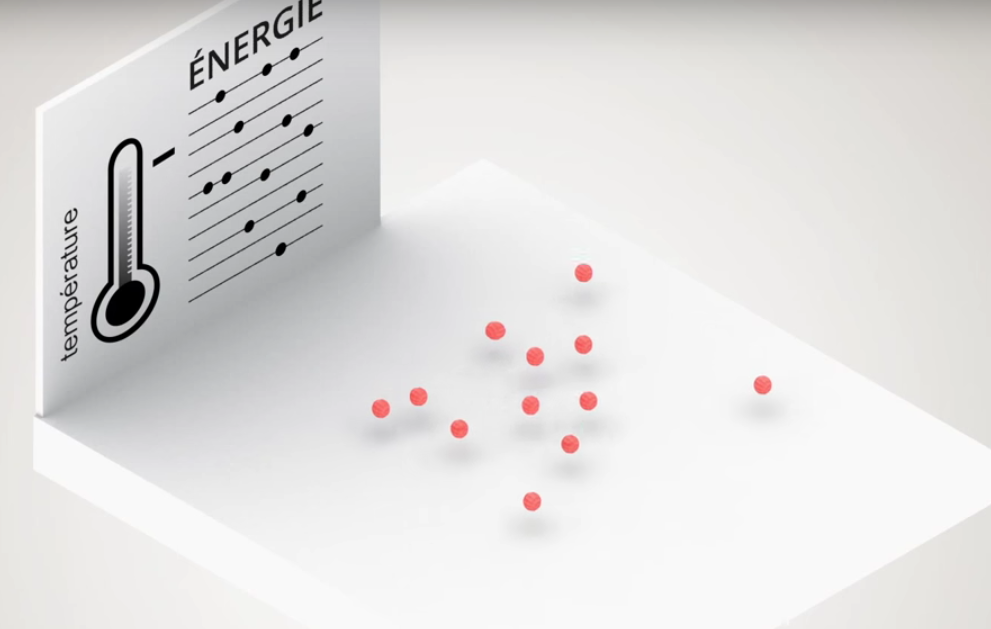
\includegraphics[scale=0.2]{./img/IM2}
		\caption{Un ensemble de bosons dans un puits 2D à une température ambiante}
	\end{center}
\end{figure}

\begin{figure}[H]
	\begin{center}
		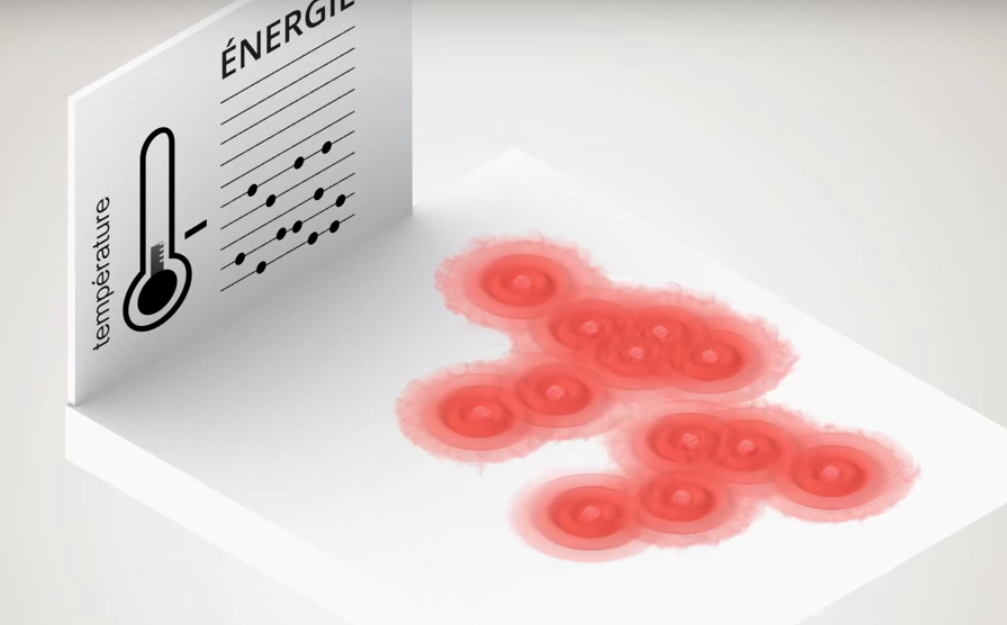
\includegraphics[scale=0.2]{./img/IM3}
		\caption{Un ensemble de bosons dans un puits 2D à une température inférieure à l'antérieure, se rapprochant de la température de Bose}
	\end{center}
\end{figure}

\begin{figure}[H]
	\begin{center}
		
\includegraphics[scale=0.2]{./img/IM4}
		\caption{Un ensemble de bosons dans un puits 2D à une température extrêmement proche de celle de Bose}
	\end{center}
\end{figure}

\subsubsection*{Les photons}

Une petite incision sur le cas des photons. Ce sont des bosons on peut donc écrire:
$$\bar{n}=\frac{1}{e^{\beta (\epsilon_0 -\mu)}-1}$$
Cependant ils existe de multiples phénomènes qui vont faire varier le nombre de particules. Cependant on peut essayer de calculer le nombre moyen optimum de photons (dans une enceinte de volume fini et en contact avec un thermostat) et minimisant l'énergie libre. $\frac{\partial F}{\partial N}=0$ on donc $\mu=0$. \\
On obtiens ensuite facilement les relations ci-dessous en prenant en compte que $E_i=n_i\hbar \omega_i$ et que l'on néglige les énergies de point zéro.
$$\bar{n}_{phot,i}=\frac{1}{e^{\beta (\beta \hbar \omega_i)}-1}$$
$$\langle \epsilon_i \rangle=\bar{n}_{phot,i}\hbar \omega_i=\frac{\hbar \omega_i}{e^{\beta (\beta \hbar \omega_i)}-1}$$


\section{De l'approximation classique à la limite classique}


On traite ici de la différence entre ces 2 notions qui peuvent porter confusion.

\begin{itemize}[label=\ding{69}]

	\item Approximation Classique

	\begin{itemize}[label=\ding{69}]

		 \item Utilités:
		 On peut traiter l'énergie comme un continuum. On peut remplacer les sommes discrètes par des intégrales
		 \item Conditions d'application:
		 $kT>> \frac{\hbar^2 \pi^2}{2mL^2}$ et molécules mono-atomiques car sinon d'autres paramètres sont à prendre en compte dans le calcul de l'énergie.

	\end{itemize}


	\item Limite classique

	\begin{itemize}[label=\ding{69}]

		 \item Utilités:
		 Elle permet de négliger le caractère quantique, on confond par exemple la statistique de B-E et F-D.
		 \item Conditions d'application:
		$$\lambda<<n^{-1/3}$$

	 \end{itemize}

\end{itemize}